\usepackage{dirtree}
\usepackage{listings}
\lstset{basicstyle=\ttfamily}

\usepackage{tikz}
\usetikzlibrary{graphs,graphdrawing,arrows.meta,positioning}
\usegdlibrary{trees}
\tikzset{branch/.style={green!70!black},tag/.style={yellow!85!black}}

\usetheme{Madrid}
\usecolortheme{seahorse}


\graphicspath{{./images/}}

%Use itemize rather than enumerate for \note[item].
%From https://tex.stackexchange.com/a/28969
\AtBeginNote{%
	\let\enumerate\itemize%
	\let\endenumerate\enditemize%
}

%A command for unnumbered footnotes.
%From https://tex.stackexchange.com/a/30723
\makeatletter
\def\blfootnote{\gdef\@thefnmark{}\@footnotetext}
\makeatother

%\vdots with appropriate spacing for use outside a matrix.
%From https://tex.stackexchange.com/a/112212
\makeatletter
\DeclareRobustCommand{\rvdots}{%
	\vbox{
		\baselineskip4\p@\lineskiplimit\z@
		\kern-\p@
		\hbox{.}\hbox{.}\hbox{.}
	}}
\makeatother

\newcommand\dircomm[1]{\hspace{0.5em}\textrm{#1}}
\newcommand\dircommcol[1]{\dircomm{\textcolor{blue}{#1}}}

\title{An Introduction to Git}
\author{Christopher Brown}
\date{}

\begin{document}

\begin{frame}
	\titlepage
	
	\note[item]{
		I'm going to teach this over several sessions.
		Hopefully the first session will teach enough to just spin up a Git repository and start making commits.
		But if that's all you ever do, you're missing out on most of the benefits that version control will give you.
		So subsequent sessions will focus on how to get the most out of Git, and use it to be more productive.
	}
\end{frame}

\part{Prerequisites}

\begin{frame}
	\partpage
	
	\note[item]{
		Before we start looking at Git, there're some prerequisites we need to go over.
		
		\item
		Primarily, you'll need to know the very basics of the shell.
		We'll use Git from the command line (the shell), so it'll help to be familiar with it.
		
		\item
		There're also a few other things I'll explain the details of now, to save having to go off on tangents later.
	}
\end{frame}

\section{The Shell}

\subsection{Introduction}

\begin{frame}{Which Shell?}
	\begin{itemize}
		\item \texttt{sh}: the Bourne Shell by Stephen Bourne, 1977
		\item \texttt{bash}: the Bourne Again SHell, 1989
		\item \texttt{zsh}, \texttt{ksh}, \texttt{tcsh}, \texttt{rc}\dots
	\end{itemize}
	\texttt{bash} is default on most Linux distros.
	
	Mac OS X defaults to \texttt{zsh}.
	
	Git on Windows comes with a \texttt{bash} emulator.
	
	\note[item]{
		You might have heard of the shell called the ``terminal'' or the ``command line''.
		It's a text-based interface to your computer.
		You can use it instead of a graphical user interface (GUI).
		
		\item
		There are GUIs for Git, but it's good to know how to use it through the command line.
		
		\item
		Different shells, \texttt{bash}, \texttt{zsh}, etc.\ are mostly based on the Bourne shell.
		There are differences, but they're all similar enough that we shouldn't run into the differences here.
		
		\item
		On Linux or Mac OS X, you should be able to search for and open the ``terminal''.
		On Windows, you're looking for ``Git Bash''.
		Open it now.
	}
\end{frame}

\subsection{Navigation}

\begin{frame}{UNIX Directories}
	\begin{itemize}
		\item \texttt{/} is the root directory
		\item \texttt{cd \textasciitilde} is your user's home directory
		\begin{itemize}
			\item \texttt{/home/abc123/} on Linux
			\item \texttt{/Users/abc123/} on Mac OS X
			\item \texttt{/c/Users/abc123/} in Git Bash on Windows
		\end{itemize}
		\item \texttt{.} is the current directory
		\item \texttt{..} is the parent directory
	\end{itemize}
	Paths starting with \texttt{/} or \texttt{cd \textasciitilde} are \emph{absolute paths}.
	
	Others are \emph{relative paths}, and start from the current directory.
	
	\note[item]{
		The first thing to learn is how the directory structure is represented on the command line.
		Directories and files have \emph{paths}: a list, one inside the other, of the directories in the tree structure reaching down to them.
		Paths are separated by forward slashes.
		Windows sometimes uses backslashes, but Git Bash does it properly with forward slashes.
		
		\item
		The difference between absolute and relative paths is important in general.
		Generally, your code should use relative paths whenever possible.
		This is especially important in Git repositories.
		Suppose someone else downloads your repo: they'll have a different username, or put it in a different place, so the absolute path will be different.
		Use relative paths instead.
	}
\end{frame}

\begin{frame}{Moving Around}
	\begin{itemize}
		\item \texttt{pwd}: Print Working Directory
		\item \texttt{cd}: Change Directory
		\begin{itemize}
			\item \texttt{cd -} goes to previous directory
		\end{itemize}
		\item Right click in file manager to open command line there
	\end{itemize}
	
	\note[item]{
		At any point, your shell is in one directory: the \emph{working directory}.
		\texttt{pwd} (print working directory) will tell you which directory you're in.
		Try it now.
		
		\item
		Before we start doing anything, we'll usually want to move to the correct directory.
		We do this with \texttt{cd} (change directory).
		
		\item
		\texttt{cd} can take a relative or absolute path.
		This is when \texttt{..} to go up a directory becomes useful, and note that we can chain this or include it mid-path.
		\texttt{cd} can also take the special argument \texttt{-} to go back to the most recent working directory.
		Play around with it.
		
		\item
		You can also open the command line directly in a directory, by right-clicking in the file manager.
	}
\end{frame}

\subsection{Inspection}

\begin{frame}{Looking Around}
	\begin{itemize}
		\item \texttt{ls}: LiSt directory contents
		\begin{itemize}
			\item \texttt{ls -a} includes hidden files/directories (e.g.\ \texttt{.git}, {.gitignore})
			\item \texttt{ls -l} gives extra info
			\item \texttt{ls -al} does both
		\end{itemize}
	\end{itemize}
	
	\note[item]{
		When you're in a directory, you want to know which files are there.
		Or which directories, so you can \texttt{cd} further in.
		\texttt{ls} tells you.
		
		\item
		\texttt{ls} takes options, a.k.a. \emph{flags}.
		\texttt{-a} (all) shows hidden files and directories, which start with a dot.
		This is important, 'cause Git uses these.
		\texttt{-l} (long) shows owner, permissions, size, date, etc.
		
		\item
		A hyphen and a single letter is the convention for flags in the shell.
		We can combine options by giving them sequentially.
		A single hyphen followed by multiple letters also combines flags.
		Order doesn't matter.
		Demonstrate this.
		
		\item
		Some programs take long options: these use two hyphens followed by a word.
		We'll see these later on some Git commands.
	}
\end{frame}

\begin{frame}{Looking at Files}
	\begin{itemize}
		\item \texttt{cat}: print a file
		\item \texttt{head}: print the first 10 lines of a file
		\item \texttt{tail}: print the last 10 lines of a file
		\item \texttt{less}: open a file in the pager
	\end{itemize}
	
	\note[item]{
		There are a variety of ways we can look at the contents of a file in the command line.
		These all work within the command line, so they'll only work for text files.
		
		\item
		The names are a bit funny.
		\texttt{cat} comes from ``concatenate'', because it can print several files back-to-back.
		\texttt{less} is a better version of \texttt{more}.
	}
\end{frame}

\begin{frame}{Opening Files \& Directories}
	\begin{itemize}
		\item Open a file with the OS:
		\begin{itemize}
			\item \texttt{open} on Mac OS X
			\item \texttt{xdg-open} in Linux
			\item \texttt{start} in Git Bash on Windows
		\end{itemize}
		\item Using these on a directory opens the file manager
	\end{itemize}
	
	\note[item]{
		If you want to use your normal text editor, or work with non-text files, you can open files as though you'd double-clicked them in your file manager.
		How to do this differs by OS.
		
		\item
		You can also use these to open your file manager, which can be helpful to move or copy files if you're not familiar with doing so on the command line.
	}
\end{frame}

\subsection{Modification}

\begin{frame}{Changing Things}
	\begin{itemize}
		\item \texttt{mkdir}: MaKe DIRectory
		\item \texttt{rmdir}: ReMove empty DIRectory
		\item \texttt{touch}: create blank file, or change last modified date
		\item \texttt{cp}: CoPy a file
		\begin{itemize}
			\item \texttt{cp -r}: CoPy a directory (recursive)
		\end{itemize}
		\item \texttt{mv}: MoVe/rename a file/directory
		\item \texttt{rm}: ReMove a file
		\begin{itemize}
			\item \texttt{rm -i} asks confirmation: safer
			\item \texttt{rm -r} removes a directory and everything inside: DANGER!
		\end{itemize}
	\end{itemize}
	
	\note[item]{
		We can use all sorts of commands to create, remove, copy, or remove files or directories.
		I won't go into the details now, and you should be able to do most of this with your file manager.
		But this might be useful in future, and you might see me using these out of habit.
	}
\end{frame}

\section{Hashes}

\subsection{SHA1}

\begin{frame}{Hashing}
	\centering
	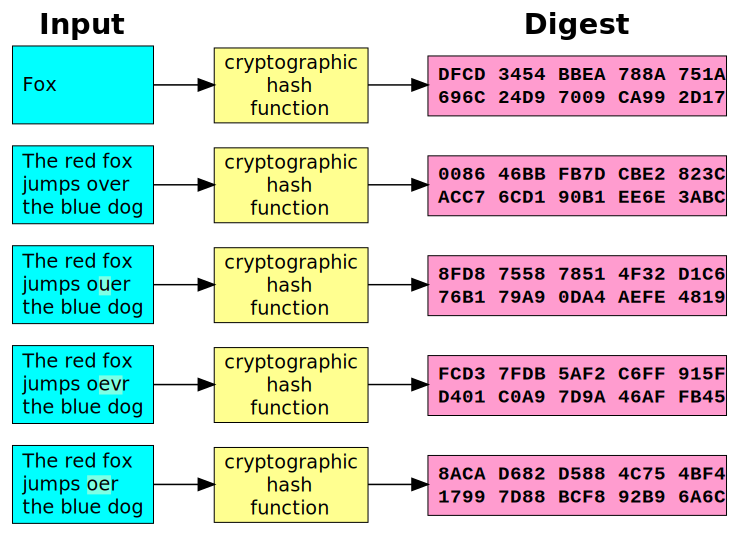
\includegraphics[width=\textwidth,height=0.8\textheight,keepaspectratio]{sha1}
	\blfootnote{Cryptographic Hash Function by Jorge Stolfi}
	
	\note[item]{
		A hash function converts some arbitrary input to a fixed-length string of seemingly-random input.
		It always converts the same input to the same output.
		But small changes in input cause large changes in output.
		
		\item
		This example uses the SHA1 hash function, the same one used by Git.
		We'll get to why Git needs this later.
		
		\item
		You can use \texttt{sha1sum} at your command line.
		(Demonstrate this a bit.)
		
		\item
		Note that you can use this hash huge files, and still get a fixed-length output.
		It's theoretically possible for two different files to give the same output, but astronomically unlikely.
	}
\end{frame}

\subsection{Uses}

\begin{frame}{Uses of Hashes}
	\begin{itemize}
		\item Checksums: checking download validity
		\item Security: storing passwords
		\item Version control: identifying versions
	\end{itemize}
	
	\note[item]{
		Hashes have a bunch of different uses.
		
		\item
		Suppose you download a huge file, and you want to know if the download got corrupted.
		The server hashes the file, and you hash the file, and you compare hashes.
		If one small bit in the file is wrong, the hash will be totally different.
		
		\item
		Websites that need a password should never store your password in plain text.
		If they did, and they got hacked, your password would be available for everyone to see.
		Instead, they store a hash of your password.
		When you submit your password, they check the hash of that against their stored hash.
		Hashes are not easily reversible, so someone who hacks the server and gets the hash can't easily get your original password.
		
		\item
		Our use is in version control.
		You can hash a file.
		Then, to check if the file's changed, you can just hash it again and check if the hash has changed.
	}
\end{frame}

\part{Introduction to Git}

\begin{frame}
	\partpage
	
	\note[item]{
		With that out of the way, it's time to start explaining Git itself.
		That said, I'll be beginning with quite a lot of motivation and background before we get into the actual commands, so bear with me.
	}
\end{frame}

\section{Terminology}

\subsection{History}

\begin{frame}{What is a Git?}
	\begin{columns}[onlytextwidth]
		\begin{column}{0.6\textwidth}
			git: An unpleasant, contemptible, or frustratingly obtuse person.\blfootnote{The Free Dictionary}
		\end{column}
		\hfill
		\begin{column}{0.4\textwidth}
			\centering
			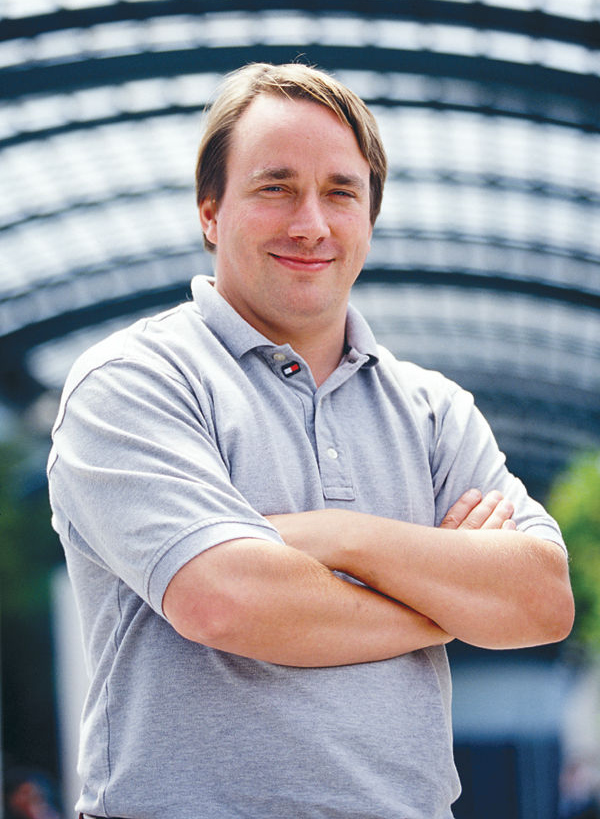
\includegraphics[width=\textwidth,height=0.8\textheight,keepaspectratio]{linus}
		\end{column}
	\end{columns}
	\blfootnote{Linus Torvalds, Linux Magazine 2002}
	
	\note[item]{
		Git is a version control system written by Linux Torvalds, the creator of Linux.
		He created it to manage the Linux kernel when the licence for the previous version control system he used was revoked.
		
		\item
		As for the name, Linus had this to say:
		``I'm an egotistical bastard, and I name all my projects after myself. First `Linux', now `git'.''
	}
\end{frame}

\subsection{Disambiguation}

\begin{frame}{Git vs GitHub}
	Git and GitHub are not the same thing!
	\medskip
	\begin{itemize}
		\item Git: version control system, runs locally
		\begin{itemize}
			\item Open source, maintained by Junio Hamano
		\end{itemize}
		\item GitHub: website and cloud server host
		\begin{itemize}
			\item Owned by Microsoft
		\end{itemize}
		\item GitLab, Bitbucket, SourceForge, etc.: other Git server hosts
	\end{itemize}
	
	\note[item]{
		This is a mistake I've heard a lot of people making, so I'm just going to clarify right now: Git and GitHub are not the same thing.
		
		\item
		Git is the version control tool.
		It's the set of commands you run on your computer.
		It's the thing originally written by Linus, and now maintained as an open source project.
		
		\item
		GitHub is a website that hosts Git repositories.
		They run a copy of Git, and serve as a place for you to store Git-managed files.
		They're not the only such host: there are dozens of commercial ones.
		You can even spin up a Git server on your own computer, and host your own.
		
		\item
		Think of Git as a file manager, and GitHub as being your friend's hard drive (or Microsoft's hard drive in this case).
		You can send files to your friend to back them up, or for them to pass on to other people.
		Meanwhile, you've still got your own copy of your file manager, and your own copy of your files.
	}
\end{frame}

\section{Motivation}

\subsection{General Use}

\begin{frame}{Why Use Git?}
	\centering
	\includegraphics[width=\textwidth,height=0.8\textheight,keepaspectratio]{phd-final}
	\blfootnote{Piled Higher and Deeper by Jorge Cham}
	
	\note[item]{
		Why do we use Git?
		The main things is that it allows us to keep different versions in a well-controlled fashion.
		It avoids the stereotypical proliferation of poorly named ``final'' versions.
		
		\item
		It's also very useful for any sort of collaborative effort.
		Have you ever done any sort of collaborative project where you're emailing files back and forth.
		Nobody can keep track of which is the most recent version.
		And if you both change a file at the same time, how do you combine the versions?
		Git handles the versioning for you, and also has a very neat algorithm for merging two sets of changes into a version with both changes.
		
		\item
		Version control is also very useful for reproducible research.
		When you share a paper, you can use version control to provide a snapshot of the code that produced it.
		Then, even if you keep working on that code, that snapshot exists for you or others to reproduce that work.
	}
\end{frame}

\subsection{Fixing Problems}

\begin{frame}{What Can Git Do?}
	\begin{itemize}
		\item What have other people changed since I last worked on this?
		\begin{itemize}
			\item \texttt{git log}
		\end{itemize}
		\item I changed some stuff, and my supervisor changed some other stuff, and I need to combine them
		\begin{itemize}
			\item \texttt{git merge}
		\end{itemize}
		\item I want to try something, but I'm worried it'll break stuff
		\begin{itemize}
			\item \texttt{git branch}
		\end{itemize}
		\item Everything I've just done has made things worse; I want to go back to how it was
		\begin{itemize}
			\item \texttt{git reset --hard} (or \texttt{git stash})
		\end{itemize}
		\item This was working fine a week ago, but now it's broken
		\begin{itemize}
			\item \texttt{git bisect}
		\end{itemize}
		\item What was I thinking when I wrote this line?
		\begin{itemize}
			\item \texttt{git blame}
		\end{itemize}
	\end{itemize}
	
	\note[item]{
		Git can do a lot more than just the standard storing and sharing of versions.
		It has a lot of benefits even just for a solo developer.
		Today, I'm going to focus mostly on just getting you working with Git.
		But next session, we'll go over some of the really helpful things you can do with it.
		
		\item
		In the meantime, here's a taste of some of the things we can do with Git.
		Have you ever found yourself in any of these situations?
		Git has commands to solve them.
	}
\end{frame}

\section{The Git Parable Pt. I}

\subsection{The Parable}

\begin{frame}{How Not To Explain Git}
	\centering
	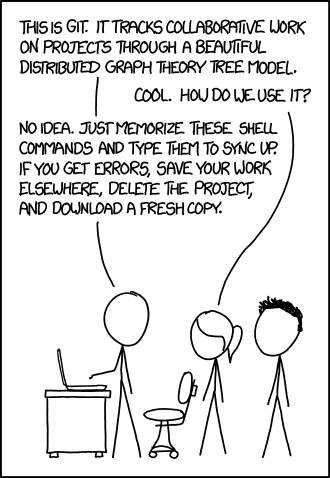
\includegraphics[width=\textwidth,height=0.8\textheight,keepaspectratio]{xkcd-git}
	\blfootnote{xkcd by Randall Munroe}
	
	\note[item]{
		A lot of people teach Git by this method: they show the standard \texttt{pull}, \texttt{add}, \texttt{commit}, \texttt{push} workflow, and leave it at that.
		The problem with doing this is that, while it allows you to work with other people who use Git, you get very little benefit from using Git that way.
		You won't understand enough to do any of the cool and useful things I just demonstrated.
	}
\end{frame}

\begin{frame}{How To Explain Git}
	The Git Parable, by Tom Preston-Werner
	\begin{itemize}
		\item \url{https://tom.preston-werner.com/2009/05/19/the-git-parable.html}
	\end{itemize}
	Suppose you only have a text editor and a file manager.
	How would you develop version control?
	
	\note[item]{
		Instead, I'm going to explain how Git actually works.
		It can appear quite complicated, so we're going to build it from the ground up.
		I'm shamelessly stealing from the best explanation of Git I've seen: ``the Git Parable'', by Tom Preston-Werner, co-founder of GitHub.
		
		\item
		The Git Parable works as follows.
		Suppose Git doesn't exist; suppose you don't have any fancy software at all.
		You've just got a text editor and a file manager, and you're setting out on a massive coding project that you need to version control.
		How, with just your text editor and file manager, would you control your versions?
	}
\end{frame}

\subsection{Snapshots}

\begin{frame}{Snapshots}
	\begin{columns}[onlytextwidth]
		\begin{column}{0.33\textwidth}
			\centering
			\includegraphics[width=\textwidth,height=0.8\textheight,keepaspectratio]{snapshot-2001-01-19}
			2001-01-19
		\end{column}
		\hfill
		\begin{column}{0.33\textwidth}
			\centering
			\includegraphics[width=\textwidth,height=0.8\textheight,keepaspectratio]{snapshot-2004-05-29}
			2004-05-29
		\end{column}
		\hfill
		\begin{column}{0.33\textwidth}
			\centering
			\includegraphics[width=\textwidth,height=0.8\textheight,keepaspectratio]{snapshot-2008-10-18}
			2008-10-18
		\end{column}
	\end{columns}
	
	\note[item]{
		Alfred is a friend of yours who works at a ``Special Moments'' photo boutique.
		He tells you the story of a woman who brings her child in for a portrait on the same day every year.
		``She brings the photos from all the past years with her,'' Alfred tells you.
		``She likes to remember what her daughter was like at each different stage, as if the snapshots really let her move back and forth in time to those saved memories.''
		
		\item
		This gives you an idea.
		Snapshots, like save points in a video game, are what you want for your version control system.
		What if you could take snapshots of your codebase at any time and resurrect that code on demand?
		So you go running back to your computer and start working.
	}
\end{frame}

\begin{frame}[t]{Snapshot Directories}
	\only<+|handout:0>{
		\dirtree{%
			.1 project.
			.2 working.
			.3 download-genomes.R.
			.3 read-genomes.R.
		}
	}
	\only<+|handout:0>{
		\dirtree{%
			.1 project.
			.2 working.
			.3 download-genomes.R.
			.3 read-genomes.R.
			.2 snapshot-0.
			.3 download-genomes.R.
			.3 read-genomes.R.
		}
	}
	\only<+|handout:0>{
		\dirtree{%
			.1 project.
			.2 working.
			.3 download-genomes.R.
			.3 read-genomes.R.
			.2 snapshot-0.
			.3 download-genomes.R.
			.3 read-genomes.R.
			.2 snapshot-1.
			.3 download-genomes.R.
			.3 read-genomes.R.
		}
	}
	\only<+>{
		\dirtree{%
			.1 project.
			.2 working.
			.3 download-genomes.R.
			.3 read-genomes.R.
			.2 snapshot-0.
			.3 message.
			.3 download-genomes.R.
			.3 read-genomes.R.
			.2 snapshot-1.
			.3 message.
			.3 download-genomes.R.
			.3 read-genomes.R.
		}
	}
	
	\note[item]{
		You begin with a \texttt{project} directory.
		This will contain everything for the project, including all your versions.
		
		\item
		Within this, you create a \texttt{working} directory.
		This will contain all the code, however many files that is.
		This is the version you'll change as you work.
		
		\item
		When you've a written a feature, you make sure everything's saved, then copy the entire \texttt{working} directory to \texttt{snapshot-0}.
		You make sure never to change any of the files in \texttt{snapshot-0}; they're permanently fixed.
		You keep making changes in \texttt{working}, and when you're done with the next feature, you again copy the whole of \texttt{working} to \texttt{snapshot-1}.
		
		\item
		These numbers aren't very helpful, so you create a file called \texttt{message} in each snapshot directory.
		This records the date of creation, and a summary of the work you did in that snapshot.
	}
\end{frame}

\begin{frame}[fragile]{Commit Messages}
	\texttt{snapshot-0/message}
	\begin{lstlisting}[frame=single,tabsize=4,gobble=8]
		2023-08-13T11:02:29+10:00
		Add download() to download FASTA files.
	\end{lstlisting}
	\bigskip
	\texttt{snapshot-1/message}
	\begin{lstlisting}[frame=single,tabsize=4,gobble=8]
		2023-08-13T11:27:47+10:00
		Refactor download() to use web_history.
		
		This should allow larger values of retmax,
		speeding up the download.
	\end{lstlisting}
	
	\note[item]{
		The message files for a couple of snapshots might look like this, with a date and time of creation, and a summary of what work was done to create them.
		
		\item
		I've written the date and time in ISO format: year, month, day, 24 hour time, and time zone offset.
		Git actually stores them in UNIX format: the number of seconds since the beginning of 1970, plus time zone offset.
		But that's not human readable.
		
		\item
		Note that each snapshot represents a single, small unit of work.
		Per Git convention, I've written the summary messages in the imperative tense: ``do this''.
		We can use extra lines to provide extra information, such as the justification for a change.
	}
\end{frame}

\subsection{Branches}

\begin{frame}[t]{Non-Linear Development}
	\only<+|handout:0>{
		\dirtree{%
			.1 project.
			.2 working.
			.2 snapshot-0.
			.2 ....
			.2 snapshot-99.
		}
	}
	\only<+|handout:0>{
		\dirtree{%
			.1 project.
			.2 working.
			.2 snapshot-0.
			.2 ....
			.2 snapshot-99.
			.2 ....
			.2 snapshot-109.
		}
	}
	\only<+>{
		\dirtree{%
			.1 project.
			.2 working.
			.2 snapshot-0.
			.2 ....
			.2 snapshot-99.
			.2 ....
			.2 snapshot-109.
			.2 snapshot-110\dircomm{?}.
		}
	}
	\note[item]{
		So, you now have a version control system, and it's working great.
		You can jump back to any earlier version whenever you want.
		
		\item
		You keep making changes, and making snapshots, and eventually you get to \texttt{snapshot-99}.
		Happy with what you've got, you release \texttt{snapshot-99} to the general public, as release version 1.0.
		
		\item
		The public likes your software, so you set out to add new features for the next version.
		You create another ten snapshots, and soon you're at \texttt{snapshot-109}.
		
		\item
		But then the bug reports start rolling in.
		It's fine, nobody's perfect, but it turns out that people using \texttt{snapshot-99} have found some problems.
		You don't want all your new features getting in the way while you debug, so you copy the contents of \texttt{snapshot-99} into your \texttt{working} directory.
		It's a quick fix, and soon you're ready to create \texttt{snapshot-110}.
		But now you've got a problem.
		\texttt{snapshot-110} is based on \texttt{snapshot-99}, not \texttt{snapshot-109}.
	}
\end{frame}

\begin{frame}{Branches}
	\begin{columns}[onlytextwidth]
		\begin{column}{0.6\textwidth}
			\centering
			\includegraphics[width=\textwidth,height=0.75\textheight,keepaspectratio]{tree}
			\blfootnote{Winter Tree, Haslemere, by Simon Burchell}
		\end{column}
		\hfill
		\begin{column}{0.4\textwidth}
			\centering
			\newcommand\treediagram{
				\graph[tree layout,grow'=up,fresh nodes] { %fresh nodes allows duplicate node names.
					snapshot0/"snapshot-0" <- "\rvdots" <- snapshot99/"snapshot-99" <- {
						snapshot100/"snapshot-100" <- "\rvdots" <- snapshot109/"snapshot-109",
						snapshot110/"snapshot-110"
					}
				};
			}
			\begin{tikzpicture}[>={Stealth[length=4pt,width=4pt]}]
				\treediagram
			\end{tikzpicture}
		\end{column}
	\end{columns}
	
	\note[item]{
		Pondering the problem, you decide to go for a walk in nature.
		Your eyes fall upon a large tree beside the path.
		Fixing your gaze upon one twig, it's easy easy to follow it back to the base of the tree.
		From the twig to the branch it grew from, from branch to bough, bough to trunk, and then down to the roots.
		
		\item
		You realise this is the perfect model for keeping track of multiple lines of development.
		For each snapshot, you just need to keep track of which snapshot it grew from, and then following these links, you will be trace any branch right back to the root, following the whole line of development.
	}
\end{frame}

\begin{frame}[fragile]{Parents}
	\texttt{snapshot-99/message}
	\begin{lstlisting}[frame=single,tabsize=4,gobble=8]
		parent snapshot-98
		2023-08-20T09:15:16+10:00
		Update version number to 1.0.0.
	\end{lstlisting}
	
	\texttt{snapshot-100/message}
	\begin{lstlisting}[frame=single,tabsize=4,gobble=8]
		parent snapshot-99
		2023-08-21T01:00:12+10:00
		Add query() to get a list of available files.
	\end{lstlisting}
	
	\texttt{snapshot-110/message}
	\begin{lstlisting}[frame=single,tabsize=4,gobble=8]
		parent snapshot-99
		2023-08-22T06:29:05+10:00
		Fix download() failing on Windows machines.
	\end{lstlisting}
	
	\note[item]{
		So, how do you implement this?
		Simple: store the parent of each snapshot in the \texttt{message} file.
		
		\item
		This is what it might look like.
		Each \texttt{message} file now has an extra line, giving the parent.
		For now, most snapshots just use the previous number as the parent: 99's parent is 98, 100's parent is 99.
		But the parent of snapshot 110 is snapshot 99.
		
		\item
		Just this simple mechanism suffices to store the entire structure of the tree, and the entire history for any snapshot.
	}
\end{frame}

\begin{frame}{Branch Names}
	\centering
	\begin{tikzpicture}[>={Stealth[length=4pt,width=4pt]},node distance=1em]
		\onslide<+->{
			\graph[tree layout,grow'=up,fresh nodes] { %fresh nodes allows duplicate node names.
				snapshot0/"snapshot-0" <- "\rvdots" <- snapshot99/"snapshot-99" <- {
					snapshot100/"snapshot-100" <- "\rvdots" <- snapshot109/"snapshot-109",
					snapshot110/"snapshot-110"
				}
			};
		}
		\onslide<+->{
			\node[branch,right=of snapshot109] (master) {master} edge[->,branch] (snapshot109);
			\node[branch,right=of snapshot110] (v1maintenance) {v1.0-maintenance} edge[->,branch] (snapshot110);
		}
		\onslide<+->{
			\node[tag,right=of snapshot99] (v1) {v1.0.0} edge[->,tag] (snapshot99);
		}
	\end{tikzpicture}
	
	\note[item]{
		So, the code history is now a tree, and we can trace any snapshot back to the root.
		This is great; we can now have multiple lines of development at once.
		
		\item
		But there's a problem.
		If we're just looking at the list of all snapshots, how do we know which is the most recent one on each branch?
		It was fine when they were sequential: the highest number was the most recent.
		But what about now?
		
		\item
		So, we need to keep a list of the most recent snapshot for each branch.
		This is a list of pointers to snapshots, one for each branch.
		We've got two branches now.
		The one we're mostly working on and developing new features on, we'll call \texttt{master}.
		The one for fixing bugs in the release version, we'll call it \texttt{v1.0-maintenance}.
		
		\item
		While we're at it, it'd be nice to keep track of some other important snapshots, like the \texttt{snapshot-99} that we released to the public.
		We'll point at this one, and call it \texttt{v1.0.0}.
	}
\end{frame}

\begin{frame}[fragile]{Storing Branches}
	\texttt{branches}
	\begin{lstlisting}[frame=single,tabsize=4,gobble=8]
		master snapshot-109
		v1.0-maintenance snapshot-110
	\end{lstlisting}
	\bigskip
	\texttt{tags}
	\begin{lstlisting}[frame=single,tabsize=4,gobble=8]
		v1.0.0 snapshot-99
	\end{lstlisting}
	
	\note[item]{
		So, how will we store these branch pointers.
		We'll create a special file called \texttt{branches}.
		\texttt{branches} doesn't sit in \texttt{working}, or in any of the snapshots.
		It's got to live somewhere separate.
		In this parable, we'd keep it in the top level project directory.
		In practice, Git keeps it in a special \texttt{.git} directory.
		
		\item
		So we just have a file listing each branch, and which snapshot is its tip.
		Whenever we create a new snapshot on the end of a branch, we need to update this file.
		
		\item
		The other special snapshots, we'll call ``tags'', and we'll put them in another file (also called \texttt{tags}).
		Tags are exactly like branches, except that they never move.
		That snapshot will always have been the v1.0.0 release.
		
		\item
		A note:
		\texttt{master} is the default name Git will use for the first branch when you create a repository, but there's nothing special about it.
		GitHub has recently been encouraging people to call it \texttt{main} instead.
	}
\end{frame}

\section{The Git Parable Pt. II}

\subsection{Distributed}

\begin{frame}{A Sharing Problem}
	\centering
	\begin{tikzpicture}[>={Stealth[length=4pt,width=4pt]},subgraph text top=text centered,subgraph nodes={font=\bfseries}]
		\graph[fresh nodes,tree layout,grow'=up] {
			you/You[draw] // {
				snapshot0/"snapshot-0" <- "\rvdots" <- snapshot111/"snapshot-111" <- {
					snapshot112/"snapshot-112" <- snapshot114/"snapshot-114" <- snapshot115/"snapshot-115",
					snapshot113/"snapshot-113"
				}
			},
			zoe/Zoe[draw] // {
				snapshot0/"snapshot-0" <- "\rvdots" <- snapshot111/"snapshot-111" <- {
					snapshot112/"snapshot-112",
					snapshot113/"snapshot-113" <- snapshot114/"snapshot-114" <- snapshot115/"snapshot-115"
				}
			}
		};
	\end{tikzpicture}
	
	\note[item]{
		So far, you've been working by yourself.
		But that gets lonely.
		Thankfully, you've got a friend called Zoe, and she wants to help you.
		You're liking your version control system, so you send her the whole thing.
		You just email her the entire project directory, working, snapshots, branches and tags files, and all.
		Then Zoe catches a flight to Patagonia and you don't hear from her for a week.
		
		\item
		When she gets back, you notice a problem.
		You've both been coding, and making new snapshots.
		But you're both using the same numbering system, so now you both have snapshots called \texttt{snapshot-114}, \texttt{snapshot-115}, etc.\ but with different code in them.
		You can't copy her snapshots without overwriting yours.
		And even if you could, you'd have no idea who wrote which code.
	}
\end{frame}

\begin{frame}[fragile]{Attributing Blame}
	\texttt{snapshot-114/message}
	\begin{lstlisting}[frame=single,tabsize=4,gobble=8]
		parent snapshot-110
		Christopher Brown <pyrrhicpachyderm@gmail.com>
		2023-08-22T13:09:24+10:00
		Retry downloads on 5xx HTTP errors.
		
		HTTP error codes 500 to 511 are failures on
		valid requests. They may occur erratically,
		so just retry the download.
	\end{lstlisting}
	
	\note[item]{
		Not knowing who wrote what is thankfully easy to solve.
		You add the author's name and email address to every \texttt{message} file.
	}
\end{frame}

\begin{frame}[fragile]{The Return of Hashing}
	\texttt{6d97fcee39f983edc17e304db8381ad3174c15d9/message}
	\begin{lstlisting}[frame=single,tabsize=4,gobble=8]
		Christopher Brown <pyrrhicpachyderm@gmail.com>
		2023-08-13T11:02:29+10:00
		Add download() to download FASTA files.
	\end{lstlisting}
	\medskip
	\texttt{edd9a01a7b0255754b07e57055cafd3f3cdea3b5/message}
	\begin{lstlisting}[frame=single,tabsize=4,gobble=8]
		parent 6d97fcee39f983edc17e304db8381ad3174c15d9
		Christopher Brown <pyrrhicpachyderm@gmail.com>
		2023-08-13T11:27:47+10:00
		Refactor download() to use web_history.
		
		This should allow larger values of retmax,
		speeding up the download.
	\end{lstlisting}
	
	\note[item]{
		The other problem---two snapshots having the same name---is more troublesome.
		Thankfully, you recently learned about hashing (remember that?), and you realise it presents the answer to your problems!
		Instead of calling a snapshot \texttt{snapshot-0}, you hash its \texttt{message} file, and use the hash of that as the snapshot name.
		
		\item
		Here, we've done this to the first two snapshots, previous \texttt{snapshot-0} and \texttt{snapshot-1}.
		The first \texttt{message} file hashes to give the string that forms the new snapshot name.
		We then use this snapshot name as the parent for the next snapshot, and hash that, \texttt{message} to get the name for that snapshot.
		
		\item
		Remember how a hash changes totally if any part of the contents changes?
		So two snapshots will only get the same name if they're created at the same time, by the same person, with the same summary.
	}
\end{frame}

\begin{frame}{Recombining}
	\centering
	\begin{tikzpicture}[>={Stealth[length=4pt,width=4pt]},subgraph text top=text centered,subgraph nodes={font=\bfseries}]
		\graph[fresh nodes,tree layout,grow'=up] {
			you/You[draw] // {
				6d97fce <- "\rvdots" <- 2de04ad <- {
					4b36dc9 <- 2138c74 <- 367d5d5,
					2a2b6cf
				}
			},
			combined/Combined[draw] // {
				6d97fce <- "\rvdots" <- 2de04ad <- {
					4b36dc9 <- 2138c74 <- 367d5d5,
					2a2b6cf <- 3603f71 <- 2a2b6cf
				}
			},
			zoe/Zoe[draw] // {
				6d97fce <- "\rvdots" <- 2de04ad <- {
					4b36dc9,
					2a2b6cf <- 3603f71 <- 2a2b6cf
				}
			}
		};
		\path (you) edge[->,red] (combined);
		\path (zoe) edge[->,red] (combined);
	\end{tikzpicture}
	
	\note[item]{
		Now that you and Zoe have renamed all your snapshots, you can merrily combine your repositories, because none of her snapshots have the same name as any of yours.
		You can just copy all of her snapshots into your \texttt{project} directory, and vice versa, and there won't be any collisions or confusion; you'll both have a copy of one another's work.
		
		\item
		This point is important, so it's worth reiterating.
		The hash of a snapshot uniquely identifies it (and its parent).
		Thus, entire snapshots can be passed around between different computers without losing their identity, or their place in the history tree.
	}
\end{frame}

\begin{frame}{Distributed}
	Advantages of a distributed system:
	\begin{itemize}
		\item Can work offline
		\item Can keep things private
		\item No single point of failure
	\end{itemize}
	
	\note[item]{
		Note that this is a distributed system.
		Everybody has their own copy of the repository.
		There are a number of advantages to this, over the centralised systems that some other version control systems use.
		
		\item
		You can do all your work offline.
		Zoe spends a lot of time flying around to different countries, with spotty internet access, so she appreciates this.
		it also makes things much faster, 'cause you don't need to talk to a server every time you want to do something.
		You only need the internet to share your work.
		
		\item
		You can also choose to keep some of your work private.
		Everything's fine if you decide not to share certain snapshots or branches with Zoe.
		
		\item
		Note that we haven't invoked GitHub here.
		You and Zoe can keep emailing snapshots to one another, with no need for a central host.
		But if you do use GitHub, it doesn't matter if GitHub goes bankrupt and vanishes.
		Everyone's got a copy, so everyone's got a backup.
	}
\end{frame}

\subsection{Merging}

\begin{frame}{Another Sharing Problem}
	\centering
	\begin{columns}
		\begin{column}{0.5\textwidth}
			\centering
			\begin{tikzpicture}[>={Stealth[length=4pt,width=4pt]},subgraph text top=text centered,subgraph nodes={font=\bfseries},node distance=1em]
				\graph[fresh nodes,tree layout,grow'=up] {
					you/You[draw,minimum width=12em] // {
						6d97fce <- "\rvdots" <- 168cf4c <- e46f258 <- 0f63002
					}
				};
				\node[branch,right=of 0f63002] (you math) {math} edge[->,branch] (0f63002);
			\end{tikzpicture}
		\end{column}
		\hfill
		\begin{column}{0.5\textwidth}
			\centering
			\begin{tikzpicture}[>={Stealth[length=4pt,width=4pt]},subgraph text top=text centered,subgraph nodes={font=\bfseries},node distance=1em]
				\graph[fresh nodes,tree layout,grow'=up] {
					zoe/Zoe[draw,minimum width=12em] // {
						6d97fce <- "\rvdots" <- 168cf4c <- 9d378db <- 6146273
					}
				};
				\node[branch,right=of 6146273] (zoe math) {math} edge[->,branch] (6146273);
			\end{tikzpicture}
		\end{column}
	\end{columns}
	
	\note[item]{
		Soon enough, you run into another issue.
		So far, when you've been recombining your histories, your snapshots have been separate.
		You can build on her snapshots, and vice versa.
		But what if you both work simultaneously.
		
		\item
		You've been working on the \texttt{math} branch, and you've added a function that generates magic numbers.
		But Zoe's also been working on the \texttt{math} branch, and she's added a function that generates primes.
		You like both of these features, and want to put them both in the next release.
		So what do you do?
		
		\item
		You've both just added stuff, so it's easy enough to edit the relevant file to have both your changes.
		But then when you come to create the next snapshot, you've a dilemma.
		Which snapshot is the parent?
		Yours, or Zoe's?
	}
\end{frame}

\begin{frame}[fragile]{Two Parents}
	\texttt{674dfe8646d3eeb4d2a9cc20fead1495f794a1a5/message}
	\begin{lstlisting}[frame=single,tabsize=4,gobble=8]
		parent 0f63002a0f7b9e3bebe04ea50a3fd83eee3d39e6
		parent 614627384c20bcf8d038320be8fb4c58a9b83526
		Christopher Brown <pyrrhicpachyderm@gmail.com>
		2023-08-13T15:01:49+10:00
		Merge pyrrhic/math and zoe/math.
	\end{lstlisting}
	
	\note[item]{
		It's an easy enough answer.
		It contains code from both snapshots, so both snapshots have to be parents.
		You just add an extra line to its \texttt{message} file.
		This snapshot has two parents.
		
		\item
		The actual text of the message isn't very important here.
		You've not done any actual work in this snapshot; it's just combining two previous pieces of work.
	}
\end{frame}

\begin{frame}{A Twined Tree}
	\centering
	\begin{tikzpicture}[>={Stealth[length=4pt,width=4pt]},subgraph text top=text centered,subgraph nodes={font=\bfseries},node distance=1em]
		\graph[fresh nodes,tree layout,grow'=up] {
			combined/Combined[draw,minimum width=16em] // {
				6d97fce <- "\rvdots" <- 168cf4c <- {
					e46f258 <- 0f63002,
					9d378db <- 6146273
				} <- 674dfe8
			}
		};
		\node[branch,right=of 674dfe8] (combined math) {math} edge[->,branch] (674dfe8);
	\end{tikzpicture}
	
	\note[item]{
		Now your history looks like this.
		It's not a tree anymore (but it's still a directed acyclic graph).
		
		\item
		You can pass all your snapshots, and the new merge snapshot, over to Zoe, and now both your histories look the same.
		
		\item
		Now, in this parable, you've had to manually copy your changes and Zoe's changes into the same file to prepare this merge snapshot.
		In reality, Git has a lot of very clever tools to do most of that work for you, and you'll only have to intervene manually in the most complicated of cases.
		But we'll cover more of that next time.
	}
\end{frame}

\subsection{Rewriting History}

\begin{frame}{Mistakes Were Made}
	\centering
	\begin{tikzpicture}[>={Stealth[length=4pt,width=4pt]},subgraph text top=text centered,subgraph nodes={font=\bfseries},node distance=1em]
		\graph[fresh nodes,tree layout,grow'=up] {
			6d97fce <- "\rvdots" <- 4435b31 <- 6146273[red] <- 819c08e <- 1854c54
		};
		\node[branch,right=of 4435b31] (master) {master} edge[->,branch] (4435b31);
		\node[branch,right=of 1854c54] (drunk) {drunk} edge[->,branch] (1854c54);
	\end{tikzpicture}
	
	\note[item]{
		So, like all good developers, you like to keep your code clean and well organised.
		And now that you're also storing all the history of your code, this extends to wanting to keep the history well groomed as well.
		Unfortunately, you had a few too many pints at the pub last night, then came home to your computer and started coding.
		You've produced a few snapshots along the way, and looking at them in the cold light of morning, you're cringing a little.
		
		\item
		You've at least confined your mistakes to the \texttt{drunk} branch.
		You could just forget about that branch; you don't have to touch it again if you don't want to.
		But surprisingly enough, the code itself is good.
		But you made a lot of mistakes in this snapshot in red, and only fixed them later.
		
		\item
		You'd like to keep the code in the last snapshot here, but you don't want all your mistakes immortalised for posterity.
		What can you do?
	}
\end{frame}

\begin{frame}{Again, But Cleanly}
	\centering
	\begin{tikzpicture}[>={Stealth[length=4pt,width=4pt]},subgraph text top=text centered,subgraph nodes={font=\bfseries},node distance=1em]
		\graph[fresh nodes,tree layout,grow'=up] {
			6d97fce <- "\rvdots" <- 4435b31 <- {
				6146273[red] <- 819c08e <- 1854c54,
				40119c8 <- 13b7d9c
			}
		};
		\node[branch,right=of 4435b31] (master) {master} edge[->,branch] (4435b31);
		\node[branch,right=of 13b7d9c] (drunk) {drunk} edge[->,branch] (13b7d9c);
	\end{tikzpicture}
	
	\note[item]{
		What you can do, is you can create another set of snapshots, making the same changes to the code, but how you wish you'd done it.
		Then you just go into your \texttt{branches} files, and point the \texttt{drunk} branch at your new snapshot instead.
		Note that the snapshots at the tips here have exactly the same content in the files.
		But because they have different parents and different times, they have different hashes.
		
		\item
		Now you can send this snapshot to Zoe, and so you still get your good code.
		But you never have to send her those other three snapshots, you can bury your embarrassment in the depths of your hard drive.
		The snapshots still exist, but there's no branch pointing to them, so you're unlikely to ever stumble across them.
	}
\end{frame}

\subsection{Staging Area}

\begin{frame}{Too Many Changes At Once}
	Bad commit messages:
	\begin{itemize}
		\item Add everything I wrote on Tuesday morning.
		\item Change the query, download, and read functions.
		\item Rewrite the whole math module.
	\end{itemize}
	
	\note[item]{
		There's another obstacle to keeping a well-groomed history: putting too many changes in one snapshot.
		It's a very easy mistake to make.
		
		\item
		Maybe you've just got really in the zone, and you've been hammering away at the keyboard all morning.
		You've written three new features, but you've forgotten to make any snapshots.
		
		\item
		Or suppose you go to change the \texttt{read()} function, but the change you want to make requires you to download things in a different format.
		So you change the \texttt{download()} function to handle the new format.
		But doing so also required making the \texttt{query()} function handle the new format.
		By the time you finished the change you set out to make to the \texttt{read()} function, you've actually made three different changes.
		
		\item
		In both these cases, it would be useful if each snapshot represented a discrete change, so that you can look at them in future.
		So you cant just copy your whole \texttt{working} directory to make a snapshot.
	}
\end{frame}

\begin{frame}[t]{Staging Area}
	\only<+|handout:0>{
		\dirtree{%
			.1 project.
			.2 working.
			.3 script.R\dircommcol{v123}.
			.2 staging.
			.2 6d97fcee39f983edc17e304db8381ad3174c15d9.
			.3 script.R\dircommcol{v1}.
		}
	}
	\only<+|handout:0>{
		\dirtree{%
			.1 project.
			.2 working.
			.3 script.R\dircommcol{v123}.
			.2 staging.
			.3 script.R\dircommcol{v1}.
			.2 6d97fcee39f983edc17e304db8381ad3174c15d9.
			.3 script.R\dircommcol{v1}.
		}
	}
	\only<+|handout:0>{
		\dirtree{%
			.1 project.
			.2 working.
			.3 script.R\dircommcol{v123}.
			.2 staging.
			.3 script.R\dircommcol{v12}.
			.2 6d97fcee39f983edc17e304db8381ad3174c15d9.
			.3 script.R\dircommcol{v1}.
		}
	}
	\only<+|handout:0>{
		\dirtree{%
			.1 project.
			.2 working.
			.3 script.R\dircommcol{v123}.
			.2 staging.
			.3 script.R\dircommcol{v12}.
			.2 6d97fcee39f983edc17e304db8381ad3174c15d9.
			.3 script.R\dircommcol{v1}.
			.2 864e37b35a26665ab8d6cfc595f6e4bd50e202c3.
			.3 script.R\dircommcol{v12}.
		}
	}
	\only<+|handout:0>{
		\dirtree{%
			.1 project.
			.2 working.
			.3 script.R\dircommcol{v123}.
			.2 staging.
			.3 script.R\dircommcol{v123}.
			.2 6d97fcee39f983edc17e304db8381ad3174c15d9.
			.3 script.R\dircommcol{v1}.
			.2 864e37b35a26665ab8d6cfc595f6e4bd50e202c3.
			.3 script.R\dircommcol{v12}.
		}
	}
	\only<+>{
		\dirtree{%
			.1 project.
			.2 working.
			.3 script.R\dircommcol{v123}.
			.2 staging.
			.3 script.R\dircommcol{v123}.
			.2 6d97fcee39f983edc17e304db8381ad3174c15d9.
			.3 script.R\dircommcol{v1}.
			.2 864e37b35a26665ab8d6cfc595f6e4bd50e202c3.
			.3 script.R\dircommcol{v12}.
			.2 b23984e16bfc5fc7c0df1de6a9a6f4d25d9e1cb8.
			.3 script.R\dircommcol{v123}.
		}
	}
	
	\note[item]{
		The solution is to create a staging area.
		
		\item
		You've made all your changes in the \texttt{working} directory, but you want to make them into two separate snapshots.
		So you create a \texttt{staging} directory.
		You copy the most recent snapshot into \texttt{staging}.
		
		\item
		Then you replay the first change you want to make into \texttt{staging}.
		You create the new snapshot from \texttt{staging}, instead of \texttt{working}.
		
		\item
		Then you replay the second change into \texttt{staging}, and again make a new snapshot from that.
		
		\item
		Now your snapshots are all caught up with your working directory, but you've got nice intermediate ones, showing each change incrementally.
		
		\item
		Replaying your changes one by one into \texttt{staging} would obviously be a huge chore doing it manually like this, but again Git's got you covered; it's got commands to do it nicely for you.
	}
\end{frame}

\part{Using Git}

\begin{frame}
	\partpage
	
	\note[item]{
		That concludes the parable.
		Tom Preston-Werner's site has one more section, on how Git avoid massively bloating all over your hard drive when it's taking hundreds of full copies of all your files.
		It's quite interesting, and makes clever use of hashing again, so it might be worth you reading at some point.
		But it's very deep in the plumbing of Git, so it's beyond scope here.
		
		\item
		Besides which, it's high time we cracked open Git ourselves and started using it.
	}
\end{frame}

\section{Setting Up}

\subsection{Configuration}

\begin{frame}{Configuring Git}
	\begin{itemize}
		\item \texttt{git config --global user.name "Christopher Brown"}
		\item \texttt{git config --global user.email "pyrrhicpachyderm@gmail.com"}
		\item \texttt{git config --global core.editor "nano"}
	\end{itemize}
	
	\note[item]{
		So, you recall how Git puts your name and email address in the message files?
		It's going to need to know them.
		The first couple of lines should set them; just use yours instead of mine.
		
		\item
		It's up to you whether you use your personal email or your institutional email.
		It'll probably never get used for anything.
		Its inclusion is largely a holdover from the days when developer were emailing one another source code, but you'll probably be using GitHub, which keeps track of your email separately from Git.
		I use my personal email because I won't have to change it every few years, and because half of what I do with Git is personal projects anyway.
		
		\item
		The third line sets up which editor you want to use to write commit messages, and for a few other purposes.
		I really like \texttt{nano} for this purpose, for a few reasons.
		I'm not sure if \texttt{nano} comes installed with Git Bash on Windows, so we may need to change this later, but there are other options.
	}
\end{frame}

\begin{frame}{Configuring R}
	\footnotesize
	\begin{itemize}
		\item \texttt{echo 'export PATH="/c/Program~Files/R/R-4.3.1/bin:\$PATH"' >> \textasciitilde/.bash\_profile}
		\item Close and reopen the terminal.
		\item \texttt{R --version}
		\item \texttt{R.exe --version}
	\end{itemize}
	
	\note[item]{
		It's not strictly necessary to make Git work, but I'm going to use some examples in R here, and it would be great if you could run them.
		Git Bash doesn't know where to find the copy of R you've got installed if you're running Windows, so we need to tell it.
		If you're not running Windows, just run \texttt{R --version}, and it should work.
		
		\item
		If you are running Windows, first you need to find where your R executable is located.
		It should look like on the slides, but you might have a different version.
		Then, run the first line, changing the version number if you need.
		Be careful to type all the special characters correctly, including the single and double quotes.
		Close your terminal and open it again, then one of the last two lines should work.
	}
\end{frame}

\subsection{Initialisation}

\begin{frame}{\texttt{git init}}
	\begin{itemize}
		\item \texttt{mkdir project}
		\item \texttt{cd project}
		\item \texttt{git init}
	\end{itemize}
	
	\note[item]{
		It's time to create a repository!
		Pick somewhere you want to create the repository.
		Either open a terminal there from the file manager or \texttt{cd} there.
		
		\item
		First, we create a directory to contain our repository.
		I'm just going to call it \texttt{project}.
		Feel free to come up with a different name: maybe \texttt{git-tutorial}.
		Don't use a space, though, use a hyphen, or an underscore.
		
		\item
		Then, we \texttt{cd} into that directory.
		
		\item
		Finally, we initialise a Git repository.
		This won't have any immediately obvious effect.
	}
\end{frame}

\begin{frame}{\texttt{git status}}
	\begin{itemize}
		\item \texttt{git status}
	\end{itemize}
	
	\note[item]{
		We've got a Git repository.
		Let's take stock.
		Run \texttt{git status}.
		
		\item
		We're on branch \texttt{master}, 'cause that's the default.
		We've not got any commits yet.
		We've been calling them snapshots throughout the parable, but Git calls them commits, and we're going to use that terminology going forwards.
		And it tells us we've got nothing to commit; unsurprising, as we've got no files yet.
		
		\item
		This command gets its own slide to itself because it's your lifeline.
		If you're ever confused, or you've forgotten where you were, run this.
		It'll tell you what's going on.
	}
\end{frame}

\begin{frame}{A Peek at the Plumbing}
	\begin{itemize}
		\item \texttt{ls}
		\item \texttt{ls -a}
		\item \texttt{ls .git}
	\end{itemize}
	
	\note[item]{
		So, what did \texttt{git init} even do?
		If we list files, we don't see anything.
		
		\item
		If you list \emph{all} files, you'd see a directory called \texttt{.git}.
		Files and directories beginning with a dot are hidden in UNIX systems, so we needed the flag to see this.
		If we give \texttt{ls} a directory, it will list things in that directory.
		Let's take a peek inside \texttt{.git}.
		
		\item
		\texttt{.git} is where Git keeps everything it does.
		All your snapshots, all your message files, your lists of branches and tags, and your staging area will all live inside \texttt{.git}.
		The rest of the project directory is all your working area.
	}
\end{frame}

\section{Workflow}

\subsection{Initial Commit}

\begin{frame}{The First File}
	\begin{itemize}
		\item \texttt{touch script.R}
		\item Open in a text editor:
		\begin{itemize}
			\item Mac OS X: \texttt{open script.R}
			\item Linux: \texttt{xdg-open script.R}
			\item Git Bash (Windows): \texttt{start script.R}
		\end{itemize}
		\item Edit (and save) the file:
		\begin{itemize}
			\item \texttt{print("Hello, world!")}
		\end{itemize}
		\item \texttt{Rscript script.R}
	\end{itemize}
	
	\note[item]{
		Now, it's time to create a file.
		If you want to go over to your file manager and do this there, feel free.
		
		\item
		If you want to keep using the terminal, then use \texttt{touch} to create the file.
		Then open the file, however you need to or your OS.
		For now, we're just going to put the simplest piece of code in our file.
		make sure you save it!
		
		\item
		Then we'll come back to our terminal, and we'll run the file, just to confirm it works.
	}
\end{frame}

\begin{frame}{\texttt{git add}}
	\begin{itemize}
		\item \texttt{git status}
		\item \texttt{git add script.R}
		\item Danger:
		\begin{itemize}
			\item \texttt{git add .}
			\item \texttt{git add -A}
		\end{itemize}
	\end{itemize}
	
	\note[item]{
		Before we go any further, let's run \texttt{git status} again, and see where we are.
		We've now got an untracked file.
		Untracked files are files that just aren't being managed by Git; Git doesn't think they're any of its business.
		If we want Git to manage it, we'll have to add it.
		
		\item
		We can do that with \texttt{git add}.
		\texttt{git add} adds files to the \emph{staging area}, which we saw at the end of the parable.
		Remember: anything that doesn't get added to the staging area doesn't go in the commit.
		As such, \texttt{git add} is one of the most common commands you'll be using.
		
		\item
		We can add \texttt{script.R} directly; that's the first line here.
		This is how I recommend you do things; I'll get into why more later.
		A lot of people introducing you to Git will show you one of the other two lines.
		These add \texttt{everything} in your working directory.
		You can quite easily make a mistake adding something you didn't want to, so despite how commonly you see these, I suggest you steer clear.
	}
\end{frame}

\begin{frame}{\texttt{git commit}}
	\begin{itemize}
		\item \texttt{git status}
		\item \texttt{git commit}
		\item \texttt{git commit -m "Add a Hello World script."}
	\end{itemize}
	
	\note[item]{
		Run \texttt{git status} again!
		We now have one file sitting in the staging area ready to be committed.
		So let's commit it.
		
		\item
		First, try typing \texttt{git commit}.
		Whether this works will depend on whether we got your editor properly configured, back when we set up your name and email address.
		If it works, it will open \texttt{nano}.
		Then you can type your commit message, save (with \texttt{Ctrl+S}) and exit (with \texttt{Ctrl+X}).
		If you exit without saving, it will abort with an empty commit message.
		
		\item
		Alternatively, you can give your commit message on the command line, with \texttt{-m}.
		The reason I suggest using the editor is because it lets you write multi-line commit messages more easily.
		
		\item
		We've already touched on some conventions for commit messages.
		Imperative tense, one short line, blank line, then a full description.
		Manually line wrap the long description if it exceeds 72 characters, and try to keep the one line short as well (under 50 characters).
	}
\end{frame}

\begin{frame}{Inspecting Our First Commit}
	\begin{itemize}
		\item \texttt{git status}
		\item \texttt{git log}
		\item \texttt{git show}
	\end{itemize}
	
	\note[item]{
		Once more, \texttt{git status}!
		Nothing to commit, working tree clean.
		The working directory is exactly the same as the tip of the current branch; nothing to report.
		
		\item
		Next, try \texttt{git log}.
		This is nearly as important a lifeline as \texttt{git status}.
		It shows you the whole history of the current branch, right back to the root.
		It's a great way of looking to see what's been done.
		
		\item
		Now, try \texttt{git show}.
		This shows us all the details for the most recent commit, including all the changes it made to files.
	}
\end{frame}

\subsection{Making Changes}

\begin{frame}{Making Changes}
	\begin{itemize}
		\item Change the file
		\item \texttt{git status}
		\item \texttt{git diff}
	\end{itemize}
	
	\note[item]{
		Make a change to the file.
		Add a line, or change an existing one.
		If you've still got your text editor open, just do it there and save it.
		
		\item
		Run \texttt{git status}.
		We've got changes that have not been staged.
		
		\item
		Run \texttt{git diff} to see the changes.
		This, the diff, is one of the best features of Git.
		You've already seen it with \texttt{git show}, but here's another instance of it.
		\texttt{git diff} by itself will tell you what's in your working directory, but not staged.
		You'll see plenty more uses for \texttt{git diff} later.
	}
\end{frame}

\begin{frame}{Adding Changes}
	\begin{itemize}
		\item \texttt{git add script.R}
		\item \texttt{git add -p}
		\item \texttt{git status}
		\item \texttt{reset}
	\end{itemize}
	
	\note[item]{
		Before we can commit our changes, we need to add them to the staging area.
		Again, we use \texttt{git add}.
		
		\item
		We can add the entire file, or even everything in the working directory, but I recommend against these.
		\texttt{git add -p} gives us an interactive choice of what to add or not.
		I \emph{always} use this: it's a great time to check that what you're adding is one cohesive change, and to proofread it.
		
		\item
		The run \texttt{git status} again.
		You can see it's gone green: it is staged and ready to commit.
		
		\item
		If we want to unstage it, we can \texttt{git reset}.
		This takes everything out of the staging area.
		We can also \texttt{git add -p} to interactively unstage things.
		
		\item
		Just make sure things are staged before you commit them.
	}
\end{frame}

\begin{frame}{Committing}
	\begin{itemize}
		\item \texttt{git commit}
	\end{itemize}
	
	\note[item]{
		Once we've added our changes, we can commit them.
		Not a lot to see here.
		
		\item
		However, if we used \texttt{git add -p} to stage just some of our changes, we can see (with \texttt{git show}) that only those changes got staged.
	}
\end{frame}

\begin{frame}{The Cycle}
	\begin{itemize}
		\item Edit files.
		\item \texttt{git add -p}
		\item \texttt{git commit}
	\end{itemize}
	
	\note[item]{
		This is how the cycle goes.
		We edit some files, we add them, and we commit them.
		
		\item
		For some people this is about all they know how to do with Git.
	}
\end{frame}

\subsection{Ignoring}

\begin{frame}[fragile]{Generated Files}
	\begin{lstlisting}[frame=single,tabsize=4,gobble=8]
		x <- rnorm(100)
		pdf("hist.pdf")
		hist(x)
		dev.off()
	\end{lstlisting}
	
	\note[item]{
		Edit your R script to contain the following.
		This generates a bunch of draws from a normal distribution, and plots a histogram.
		
		\item
		Note that before creating the histogram, we create a PDF file to save it to.
		\texttt{dev.off()} then closes the PDF file when we're done writing to it.
		This is how you save your figures if you don't use RStudio, by the way.
		
		\item
		Run it, and you should get \texttt{hist.pdf} appear in your directory.
	}
\end{frame}

\begin{frame}{Not Tracking}
	\begin{itemize}
		\item \texttt{git status}
		\item Don't do these:
		\begin{itemize}
			\item \texttt{git add .}
			\item \texttt{git add -A}
		\end{itemize}
	\end{itemize}
	
	\note[item]{
		Now, we've got this PDF file in our working directory.
		Do we want to add it to Git?
		
		\item
		No!
		This is a generated file.
		We can recreate it from the source code, so controlling it separately would be redundant.
		Worse, this one is random, so we'd get a new version every time we ran it.
		
		\item
		You don't want to add generated files to Git.
		Then the generated files and the code that generates them might get out of sync, and that gets terribly confusing.
		
		\item
		But now this untracked file is forever going to be floating around our \texttt{git status} output.
		And if we use \texttt{git add .} or \texttt{git add -A}, we'd accidentally add it to Git.
		It'd be nice if we could tell Git to just ignore it.
	}
\end{frame}

\begin{frame}[fragile]{\texttt{.gitignore}}
	\begin{itemize}
		\item \texttt{touch .gitignore}
	\end{itemize}
	\bigskip
	\texttt{.gitignore}
	\begin{lstlisting}[frame=single,tabsize=4,gobble=8]
		*.pdf
	\end{lstlisting}
	
	\note[item]{
		We can tell Git to ignore it!
		We use a \texttt{.gitignore} file.
		
		\item
		Create a \texttt{.gitignore} file and open it.
		Note that this starts with a dot, so it's a hidden file.
		
		\item
		In the \texttt{.gitignore}, we tell Git to ignore all PDF files.
		We could tell it to just ignore \texttt{hist.pdf}.
		Or we could tell it to ignore everything in a \texttt{figures/} directory.
		There are many options.
	}
\end{frame}

\subsection{Inspecting History}

\begin{frame}{Looking at History}
	\begin{itemize}
		\item Get an example repository:
		\begin{itemize}
			\item \texttt{cd ..}
			\item \texttt{git clone https://github.com/pyrrhicPachyderm/git-tutorial.git}
			\item \texttt{cd git-tutorial}
		\end{itemize}
		\item \texttt{git log}
		\item \texttt{git show 95f98c6}
	\end{itemize}
	
	\note[item]{
		So, we're beginning to get a bit of history in our repo.
		Now, suppose we want to go and have a look at it.
		
		\item
		You've already seen \texttt{git log}.
		Now it should be a bit longer.
		If it exceeds one screen in height, it'll enter a pager, and you can page up and down.
		While it's in the pager, you can type \texttt{/} to search the history.
		\texttt{n} does to the next match, and \texttt{N} to the previous.
		
		\item
		You've also seen \texttt{git log}.
		Without an argument, it shows you the most recent commit.
		But if you have a hash (probably from \texttt{git log}), then you look at a specific commit.
	}
\end{frame}

\begin{frame}{Checkout Out}
	\begin{itemize}
		\item \texttt{git checkout 95f98c6}
		\item \texttt{git checkout master}
	\end{itemize}
	
	\note[item]{
		Viewing patches and diffs is all well and good, but what if you want to go and see the full state of files at a particular commit.
		We need to check out that commit.
		
		\item
		This will change everything in our working directory to that commit.
		It will fail, and warn you, if it would overwrite any uncommitted changes, so don't worry.
		
		\item
		Checking out a particular leaves you with ``detached HEAD'', which is just a scary way of saying you're not looking at a particular branch any more.
		We can reattach our HEAD to the \texttt{master} branch by checking out the branch.
	}
\end{frame}

\begin{frame}{Refs}
	\begin{itemize}
		\item \texttt{git show HEAD}
		\item \texttt{git show master}
		\item \texttt{git show HEAD\textasciicircum}
		\item \texttt{git show HEAD\textasciicircum\textasciicircum}
		\item \texttt{git show HEAD\textasciitilde 2}
	\end{itemize}
	
	\note[item]{
		We don't always need to refer to a commit using its hash.
		We can all sorts of shortcuts.
		
		\item
		\texttt{HEAD} is whichever commit we've currently got checkout out.
		\texttt{master} is obviously the commit the master branch points to.
		\texttt{\textasciicircum} refers to the parent of a commit, and can be stacked.
		\texttt{\textasciitilde} is similar: it goes back a certain number of parents.
	}
\end{frame}

\begin{frame}{Diffs}
	\begin{itemize}
		\item \texttt{git diff}
		\item \texttt{git diff HEAD\textasciicircum 1}
		\item \texttt{git diff HEAD\textasciicircum 1 HEAD}
		\item \texttt{git diff HEAD\textasciicircum HEAD -- script.R}
	\end{itemize}
	
	\note[item]{
		While \texttt{git show} can show us the changes made by any one commit, we can actually diff any two arbitrary commits.
		Without arguments, it diffs the working directory against the index (the staging area).
		With one argument, it diffs the working directory against the given commit.
		With two arguments, it diffs the first against the second.
		Any arguments after a \texttt{--} are file names, and it looks only in those files.
		
		\item
		Note that \texttt{git diff HEAD\textasciicircum 1 HEAD} should be the same as \texttt{git show HEAD}.
	}
\end{frame}

\section{Branches}

\subsection{Splitting}

\begin{frame}{Creating Branches}
	\begin{itemize}
		\item \texttt{git branch}
		\item \texttt{git branch beta}
		\item \texttt{git branch}
		\item \texttt{git checkout -b feature}
		\item \texttt{git branch}
		\item \texttt{git checkout -b master}
	\end{itemize}
	
	\note[item]{
		We already how branching works in theory, so now let's see it in practice.
		
		\item
		\texttt{git branch} just lists branches, including pointing out which one we're on.
		
		\item
		\texttt{git branch name} creates a branch with a certain name.
		But it doesn't switch us to it, which might unhelpful.
		
		\item
		\texttt{git checkout -b name} creates a branch and checks it out.
		This can be more helpful.
		It fails if the branch already exists.
	}
\end{frame}

\begin{frame}{Switching Branches}
	\begin{itemize}
		\item \texttt{git checkout feature}
		\item \texttt{git checkout master}
	\end{itemize}
	
	\note[item]{
		To switch to another branch, it's just \texttt{git checkout}.
		We already saw this used to reattach our HEAD to the \texttt{master} branch.
		Well, it can attach our HEAD to any branch.
		
		\item
		HEAD is just another pointer, and it can either be pointing to a commit, or to a branch which in turn points to a commit.
	}
\end{frame}

\subsection{Merging}

\begin{frame}{Switching Branches}
	\begin{itemize}
		\item \texttt{git checkout master}
		\item \texttt{git merge feature}
	\end{itemize}
	
	\note[item]{
		If we want to merge two branches, we check one of them out and merge the other into it.
		
		\item
		It's a very common development paradigm that every new feature gets developed on a branch (with an appropriate name).
		Then that branch gets merged into the \texttt{master} branch when the feature's ready.
		That's what this example depicts.
	}
\end{frame}

\section{Collaborating}

\subsection{Remotes}

\begin{frame}{Setting Up a Remote}
	\begin{itemize}
		\item Create a GitHub repository.
		\item \texttt{git remote add origin https://github.com/pyrrhicPachyderm/project.git}
	\end{itemize}
	
	\note[item]{
		Now, it's time to share your files with some friends.
		
		\item
		We'll need to begin by hopping out of Git for a moment and going over to GitHub, in your browser.
		There, you can create a repository, and retrieve the URL for it.
		
		\item
		Then, come back to Git, and add it as a remote.
		All we've done is tell Git that the repository exists on GitHub.
		We've not sent anything up or down yet.
		
		\item
		You can register several remotes, under different names.
		\texttt{origin} is like \texttt{master}; it's a convention, but not required.
		It's called \texttt{origin}, 'cause it's usually where you downloaded the files from in the first place.
		Though in this case, you made them yourself, so it's less appropriate.
	}
\end{frame}

\begin{frame}{Pushing}
	\begin{itemize}
		\item \texttt{git push origin master}
		\item \texttt{git push -u origin master}
		\item \texttt{git push}
		\item \texttt{git status}
		\item \texttt{git log}
	\end{itemize}
	
	\note[item]{
		\texttt{git push} takes all your local commits on a branch and sends them up to be stored on the remote.
		In this case, you tell it you're explicitly pushing the \texttt{master} branch ti the \texttt{origin} remote.
		
		\item
		You don't want to type that every time, so \texttt{-u} tells the \texttt{master} branch to track the \texttt{origin} remote.
		From then on, just \texttt{git push} will work.
		
		\item
		Check out \texttt{git status} and \texttt{git log}; they now have some extra information.
	}
\end{frame}

\begin{frame}{Cloning}
	\begin{itemize}
		\item \texttt{cd ..}
		\item \texttt{git clone https://github.com/zoe/project.git zoe-project}
		\item \texttt{cd zoe-project}
		\item \texttt{git status}
		\item \texttt{git log}
	\end{itemize}
	
	\note[item]{
		Now that you've all pushed, it's time to look at what other people have been up to.
		
		\item
		There's a handy way to get a whole repository down from GitHub, and that's \texttt{git clone}.
		Swap with a neighbour, and clone their repository.
		We \texttt{cd} up first to keep the two repositories separate.
		
		\item
		\texttt{cd} into their repository, and look around.
	}
\end{frame}

\begin{frame}{Pulling}
	\begin{itemize}
		\item Get your neighbour to \texttt{git push}
		\item \texttt{git pull}
		\item \texttt{git log}
	\end{itemize}
	
	\note[item]{
		Now that you've got your neighbour's repository, sharing new commits is easy.
		They push, and you pull.
		
		\item
		Everyone, go back to their own repositories, make a change, add it, and push it.
		Then, go into your neighbour's repository, and pull their change.
		
		\item
		You need to do it that way around, as you won't be able to push directly to their repository unless they give you permission to.
	}
\end{frame}

\subsection{Forks}

\begin{frame}{Forking}
	\begin{itemize}
		\item On GitHub, fork your neighbour's repo.
		\item \texttt{git remote add fork https://github.com/me/zoe-project.git}
		\item \texttt{git push fork master}
	\end{itemize}
	
	\note[item]{
		As mentioned, you can't push directly to other people's repositories.
		They can go into GitHub and give you permission, if they really trust you.
		But a lot of the time, when you're contributing to a big open source project, they won't trust you that much.
		So how do you contribute?
		
		\item
		You create a fork.
		This is just another copy of the repository on GitHub, but under your name.
		You can push and pull your work to the fork, without affecting the main repo.
		
		\item
		Go to GitHub to fork your neighbour's project.
		Then add your fork as a remote for your local copy of your neighbour's repo.
		You now have two remotes: \texttt{origin}, their copy, and \texttt{fork}, your copy.
		
		\item
		Previously, we've pushed with \texttt{git push origin master}.
		Now, we can't push to \texttt{origin}, so we push to \texttt{fork}.
	}
\end{frame}

\begin{frame}{Pull Requests}
	\begin{itemize}
		\item Ask your neighbour to pull from your fork.
		\item \texttt{git remote add bob-fork https://github.com/bob/zoe-project.git}
		\item \texttt{git pull bob-fork master}
		\item \texttt{git push origin master}
	\end{itemize}
	
	\note[item]{
		So, you've made some changes to your fork.
		How do you get Zoe to make them to her original copy?
		You ask her to pull them from your fork.
		
		\item
		You may have heard of a pull request (or PR).
		GitHub has a whole system set up for automatic creation and review of pull requests.
		But a pull request is not inherently a part of Git.
		GitHub has this construct, but inherently, a pull request is just a request to pull.
		You can just as well make a ``pull request'' by tapping your neighbour on the shoulder and saying ``hey, I made a cool change, do you want to pull it?''
		
		\item
		If they do want to, they need to add your fork as a remote on their repo, and then they can just pull from it.
		Then, they can push to their own remote, and your change gets incorporated into the original version.
	}
\end{frame}

\end{document}
